\documentclass[10pt,a4paper]{article}
\usepackage[sfmath, light]{kpfonts} %police
\renewcommand{\familydefault}{\sfdefault}
\usepackage[frenchb]{babel}
\usepackage{numprint}
\usepackage[utf8]{inputenc}
\usepackage{amsmath}
\usepackage[use-aux,use-files]{xsim}
\xsimsetup{
	path=xsim
}
\usepackage{ifthen}
\usepackage{fontawesome5}
\usepackage{amsfonts}
\usepackage{amssymb}
\usepackage[locale=FR]{siunitx}
\usepackage[explicit]{titlesec}
\usepackage{ulem}
\usepackage[usenames,dvipsnames,svgnames,table]{xcolor}
\usepackage[margin=1in]{geometry}
\usepackage{enumitem}
\setlist[enumerate]{label=\textbf{\alph*)}, itemsep=1ex}
% création d'un nouveau paramètre pour les listes de type <enumerate>. Pour afficher le contenu de la liste en plusieurs colonnes, utiliser [cols=<nombre de colonne>]
\SetEnumitemKey{cols}
{
    before = \begin{multicols}{#1},
    after =  \end{multicols}
}
\usepackage{xlop}
\usepackage{pgf,tikz}
\usepackage[tikz]{bclogo}
\usepackage{tabularx}
\usepackage{tabularray}
\usepackage{tabulary}
\usepackage{multicol}
\usepackage{graphicx}
\usepackage{eurosym}%symbole euro
\usepackage{setspace}%interligne
\usepackage{tablists}%exercices sur plusieurs colonnes
\setlength{\parindent}{0pt}
\newcounter{nexo}
\setcounter{nexo}{1}


\begin{document}

Nom : \\
Prénom : \\ 
Classe : \\

\vspace{2cm}

\begin{center}
	\Huge{\textbf{DOSSIER DE RÉVISIONS}}\\
	\huge{\textbf{1ères - Fin d'année}}
\end{center}
	
\normalsize

\begin{exercise}
	Effectue les calculs ci-dessous en respectant la priorité des opérations.
			\begin{enumerate}[cols=2]
				\item $8\cdot 13-(6+12):3+11$
				\item $4\cdot (11-2)+10:5+10$
				\item $12\cdot 2-(7+9)+9:3$
				\item $12:2\cdot 13-13+17+9$
				\item $4+3\cdot 11+3:(6-5)$
				\item $5\cdot (5+1)-9$
				\item $5\cdot 2+12+11:(13-2)$
				\item $2+4:4+8\cdot 8-7$
				\item $12\cdot 4-(2+10):6+12$
				\item $5\cdot 11:5+2-4+9$
			\end{enumerate}
\end{exercise}

%%%%%%%%%%%%%%%%%%%%%%%%%%%%%%%%%%%%%%%%%%%%%%%%%%%%%%%%%%%%%%%%%%%%%%%%%%%%%%%%%%%%%%%%%%%%%%%%%%%%

\begin{exercise}
	Remplace les pointillés par le vocabulaire adéquat : \textit{diviseur} ou \textit{multiple}.
	\begin{enumerate}[cols=3]
		\item $16$ est un $\ldots$ de $4$
		\item $1$ est un $\ldots$ de $5$
		\item $5$ est un $\ldots$ de $5$
		\item $150$ est un $\ldots$ de $3$
		\item $18$ est un $\ldots$ de $3$
		\item $2$ est un $\ldots$ de $20$
		\item $0$ est un $\ldots$ de  tous les naturels
		\item $1$ est un $\ldots$ de tous les naturels
		\item $ 18$ est un $\ldots$ de $3$
		\item $5$ est un $\ldots$ de 5 et 15
		\item $6$ est un $\ldots$ de 3 et 2
		\item $1$ est un $\ldots$ de 1
	\end{enumerate}
\end{exercise}

\begin{exercise}
	Donne la nature des quadrilatères suivants. \\
	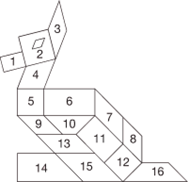
\includegraphics{img/lapinquadri.png}
\end{exercise}

\begin{exercise}
	Si possible, réduis au maximum les expressions suivantes. 
	\begin{enumerate}[cols=4]
		\item \(-b -b\)
		\item \(4a \cdot (-b)\)
		\item \(-5a\cdot (-5a)\)
		\item \(b^2 + 5b\)
		\item \(a + a + a \)
		\item \(2b - 6b + 4a\)
		\item \(b^2 - 5b^2\)
		\item \(a \cdot (-2b)\cdot (-3c)\)
		\item \(-2b + 5b\)
		\item \(2a \cdot (-5b)\)
		\item \(x-2y + 3x - 5y\)
		\item \(4x + 2xy - 10\)
	\end{enumerate}
\end{exercise}

\begin{exercise}
	Établis l'ensemble des diviseurs et l'ensemble des 5 premiers multiples des nombres ci-dessous.
	\begin{enumerate}[cols=5]
		\item $20$
		\item $150$
		\item $100$
		\item $40$
		\item $144$
		\item $16$
		\item $17$
		\item $12$
	\end{enumerate}
\end{exercise} 

\begin{exercise}
Calcule les valeurs numériques des expressions suivantes.
\begin{enumerate}[cols=2]
	\item 	\(23+t-4t\) si \(t=4\)
	\item \(3c^2-c+10\) si \(c=6\)
	\item \(3(60-p)\) si \(p=40\)
	\item \(a+2b+10ab\) si \(a=2\) et \(b=8\)
\end{enumerate}
\end{exercise}

\begin{exercise}
	Calcule les puissances suivantes.
			\begin{enumerate}[cols=6]
				\item $3^4$
				\item $-1^8$
				\item $12^2$
				\item $(-6)^2$
				\item $2^4$
				\item $(-4)^2$
				\item $1^{24}$
				\item $(-3)^3$
				\item $20^1$
				\item $(-5)^3$
				\item $-10^6$
				\item $3^0$
				\item $-2^5$
				\item $3^2$
				\item $-3^2$
				\item $(-7)^2$
				\item $(-1)^7$
				\item $17^0$
			\end{enumerate}
\end{exercise}

\begin{exercise}
	Réduis au maximum les expressions suivantes. 
	\begin{enumerate}[cols=2]
		\item \(-a + (-b – c )\)
		\item \(3\cdot (2x + 2 )\)
		\item \( – (3x - 2y) +(x - y)\)
		\item \((x + 4y)\cdot 2x\)
		\item \(-2 + (a + 4) - (-3 + a)\)
		\item \(2a \cdot (2a-5b)+12ab\)
		\item \(x²-(5x² -2x + 3)\)
		\item \((5a +5a^2)+(4 + 3a\cdot 2)\cdot 3a\)
		\item \(3+(x-5)+(x^2-5x) \)
		\item \(5a+(5-a)\cdot 4\)
		\item \(3 - 5y \cdot 2xy + 2\cdot 3x^2\cdot 5y - 10\)
		\item \(9 + 3(2a + 7) - (3a + 9)\)
	\end{enumerate}
\end{exercise}

\begin{exercise}
	Construis un parallélogramme $ABCD$ sachant que $|AC|=$ 6 cm, $|BD|=$ 4cm et $ \widehat{DMA} = 70 \degres $ \\
	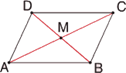
\includegraphics{img/parallelogramme.png}
\end{exercise}

\begin{exercise}
	Écris les nombres suivants sous forme d'un produit de facteurs premiers.
	\begin{enumerate}[cols=3]
		\item 180
		\item 144
		\item 50
		\item 13
		\item 24
		\item 80
		\item 128
		\item 2048
		\item 90
	\end{enumerate}
\end{exercise}

\begin{exercise}
	Range les nombres suivants par ordre croissant. \\
	\(-2,3\) \hfill 4 \hfill \(-3,2\) \hfill 4,5 \hfill \(-3,5\) \hfill \(-6,5\) \hfill 0 \hfill 1,78
\end{exercise}

\begin{exercise}
	Applique la règle des signes successifs en écrivant le calcul sans parenthèse, puis calcule.
	\begin{enumerate}[cols=3]
		\item $(-10)-(+33)$
		\item $(+68)+(-70)$
		\item $(+14)+(+65)$
		\item $(-57)-(+3)$
		\item $(+98)+(-20)$
		\item $(-47)-(+11)$
		\item $(+25)-(+17)$
		\item $(+75)+(-11)$
		\item $(+14)-(+100)$
		\item $(-20)+(+68)$
		\item $(-30) - (-15)$
		\item $(+28)-(-10)$
	\end{enumerate}
\end{exercise}

\begin{exercise}
	Que vaut \(m\) dans les équations suivantes ? Utilise les chaines d’opérations et laisse ta démarche visible.
	\begin{enumerate}[cols=2]
		\item \(4m+2=82\)
		\item \(3(m-2)=15\)
		\item \(21=3m+6\)
		\item \((3+2m)\cdot 2=22\)
	\end{enumerate}
\end{exercise}

\begin{exercise}
	Pour le cocktail d’anniversaire de Maria, il est noté ce qui suit : 

Pour 10 personnes :
-	120 cl d’eau pétillante
-	50g de sucre glace
-	20 cl de grenadine
-	1 demi citron
-	160cl de sprite

Maria compte faire ce cocktail pour les 12 personnes présentes à la fête.\\  Calcule les quantités nécessaires de chacun des aliments.
\end{exercise}

\begin{exercise}
	Par quel(s) chiffre(s) peux-tu remplacer le \faIcon{square} pour que la phrase soit correcte? 
	\begin{enumerate}[cols=2]
		\item \(84\)\faIcon{square}\(6\) est divisible par 2
		\item \(369\)\faIcon{square} est divisible par 5
		\item \(47\)\faIcon{square}\(0\) est divisible par 4
		\item \(95\)\faIcon{square}\(7\) est divisible par 3
		\item \(73\)\faIcon{square}623 est divisible par 9
		\item \(11\)\faIcon{square}5 est divisible par 125
	\end{enumerate}
\end{exercise}

\begin{exercise}
	Donne le nom de la propriété utilisée dans chacune des égalités suivantes. 
	\begin{enumerate}[cols=2]
		\item \(4 \cdot 7 = 7 \cdot 4 \)
		\item \(-9 + 1 = 1 + (-9)\)
		\item \(7 + 1 + 2 = 2 + 1 + 7 \)
		\item \(7 \cdot 0 = 0 \)
		\item \(0 + 10 = 10 \)
		\item \(3 \cdot 1 \cdot 7 = 3 \cdot 7\)
		\item \(3 \cdot 7 + 8 \cdot 9 = 8 \cdot 9 + 3 \cdot 7\)
		\item \(3 + 2 + 7 = (3 + 2) + 7\)
	\end{enumerate}
\end{exercise}

\begin{exercise}
	\emph{(Sur cette feuille)} Complète les couples de nombres pour que ceux-ci soient des nombres opposés. \\

	\((3; \ldots )\) \hfill \((-7 ; \ldots )\) \hfill \((\ldots ; 5)\) \hfill \((\ldots ; -10)\)
\end{exercise}

\begin{multicols}{2}
	\begin{exercise}
	Voici un programme de calcul dont le résultat est -15 . Retrouve le nombre de départ. \\ Justifie ta réponse. \\

	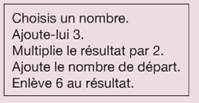
\includegraphics{img/nombreatrouver.png}
\end{exercise}

\begin{exercise}
	Les figures ci-dessous ont été dessinées à main levée, reproduis-les en respectant les mesures indiquées. \\
	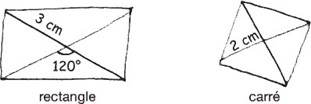
\includegraphics{img/rectanglecarre.jpg}
\end{exercise}
\end{multicols}


\begin{exercise}
	Effectue.
		\begin{enumerate}[cols=3]
		\item $8^2 - 7 \cdot (-5)$
		\item $(6^2 + 3^0)\cdot (-2)$
		\item $45-10\cdot2^2$
		\item $(4^2 - 2\cdot 3)^3$
		\item $50:5\cdot2 - 7^2$
		\item $(-5)+4^2$
		\item $5^3 - 3^3 - (-9)^2$
		\item $4+(8^2 - 3 \cdot2^2 \cdot5)$
		\item $40:5\cdot2 : 4 + 2^4$
		\item $-3 + (-2) - 5^2$
		\item $(-5+2) + (-4)^2$
		\item $18:6\cdot 2 -1^{12}$
		\item $9-5\cdot (-3)$
		\item $(-7)^2 - (3^2 + 9 \cdot 0 \cdot 1)$
		\item $4^1 - 16:2\cdot 7$
		\end{enumerate}
\end{exercise}

\begin{exercise}
	Construis un losange $ABCD$ sachant que $|\widehat{A}|= 60\degres$ et que le périmètre vaut 16 cm.
\end{exercise}

\begin{exercise}
	Calcule les pourcentages suivants. Arrondis à 2 chiffres après la virgule si besoin. 
	\begin{enumerate}[cols=3]
		\item 30\% de 120g
		\item 20\% de 366€
		\item 16\% de 1000l
		\item 75\% de 1h
		\item 86\% de 350g
		\item 25\% de 30m
		\item 97\% de 15 000€
		\item 13\% de 13kg
		\item 89\% de 400g
		\item 22\% de 8cl 
		\item 91\% de 100cm
		\item 50\% de 3h
	\end{enumerate}
\end{exercise}

\begin{exercise}
	Un étang circulaire de 4 m de rayon est bordé par une allée de 2 m de large, le tout étant clôturé par un treillis.
	\begin{multicols}{2}
		\begin{enumerate} 
			\item \emph{(Sur cette feuille)} Indique les données du problème sur la figure ci-contre. %pourquoi c'est souligné?
			\item \emph{(Sur cette feuille)} Hachure la surface de l’allée.
			\item Calcule l’aire de cette allée.
			\item Calcule la longueur du treillis.
		\end{enumerate}
		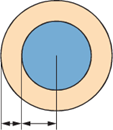
\includegraphics{img/etang.png}
	\end{multicols}
\end{exercise}

\begin{exercise}
	Factorise au maximum en utilisant la mise en évidence.
	\begin{enumerate}
		\item \(2x - 2y\)
		\item \(5ac + 5ad \)
		\item \(3 + 3a \)
		\item \(12a^3 - 8a^2b \)
		\item \(15b + 25c\)
		\item \(12 a^6b^7+ 15 a^3b^9c\)
		\item \(4 abx + 6 aby\)
		\item \(20 ab + 10a\)	
	\end{enumerate}
\end{exercise}

\begin{exercise}
	Construis un triangle sachant qu’un de ses côtés mesure 7 cm et que les angles adjacents à ce côté mesurent $45 \degres$ et $60\degres$
\end{exercise}

\begin{exercise}
	Construis un triangle sachant qu’un de ses angles mesure $80\degres$ et que les côtés qui forment cet angle mesurent 4 cm et 6 cm.
\end{exercise}

\begin{exercise}
	Lorsqu’il va chez son oculiste, Monsieur Leborgne paie 75€ pour la consultation. Sa mutuelle lui rembourse 70\% de ce montant. Sur le montant restant à sa charge après remboursement de la mutuelle, son assurance «soins de santé» lui rembourse 80\%.\\
Quel pourcentage du prix de la consultation a-t-il finalement payé ?

\end{exercise}

\begin{exercise}
	Voici la répartition des dépenses mensuelles d'un ménage. \\
	Logement : 688 € \hfill Alimentation : 539 € \hfill Habillement : 441 € \hfill
	Loisirs : 245 € \hfill Transports : 343 € \hfill 196 € \\

	Représente cette répartition à l'aide d'un diagramme circulaire.
\end{exercise}

\begin{exercise}
	Pour les cadeaux de Noël, Amélie a acheté 5 CD à la Fnac. Au moment de payer, elle a sorti un billet de 100€ de son portefeuille, mais le caissier lui a fait gentiment remarquer qu’il
manquait 12€. Calcule le prix de vente d’un CD. Laisse ta démarche visible.
\end{exercise}

\begin{exercise}
	\emph{(Sur cette feuille)} Coche d'une croix la ou les case(s) adéquate(s). 

	\begin{center}
		\begin{tblr}{
				hlines,
				vlines,
				columns={3cm, c},
				rows={1cm,m},
				row{1}={gray!40, font=\bfseries},
				column{1}={2cm, gray!40, font=\bfseries},
			}
			& est divisible par & est un diviseur de & divise & est multiple de \\
			6 \ldots 24 & & & & \\
			24 \ldots 8 & & & & \\
			1 \ldots 17 & & & & \\
			20 \ldots 20 & & & & \\
			0 \ldots 15 & & & & \\
		\end{tblr}
	\end{center}
\end{exercise}

\begin{exercise}
	Détermine la valeur de \(x\) si tu sais que le périmètre de la figure ci-dessous mesure 84 cm. \\
	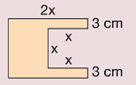
\includegraphics{img/périmetre.png}
\end{exercise}

\begin{exercise}
	En une seule étape, calcule les nouveaux prix des situations suivantes. Arrondis à 2 chiffres après la virgule si besoin.
	\begin{enumerate}[cols=2]
		\item -30\% sur 1500€
		\item +40\% sur 100€
		\item une remise de 10\% sur un montant de 500€
		\item une réduction de 28\% sur un prix de 45€
		\item un intérêt de 3\% sur un placement de 600€
		\item une TVA (21\%) à ajouter à un prix de 3,25€
		\item une augmentation de 12\% sur un prix de 155€
		\item -80\% sur 2000€
		\item -1\% sur 300€
	\end{enumerate}
\end{exercise}

\begin{multicols}{2}
	\begin{exercise}
	Le triangle ci-dessous a été dessiné à main levée. Reproduis-le en respectant les mesures puis trace ses médianes. \\
	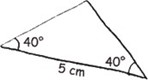
\includegraphics{img/triangleatracer.jpg}
\end{exercise}

\begin{exercise}
	Le triangle ci-dessous a été dessiné à main levée. Reproduis-le en respectant les mesures puis trace ses hauteurs. \\
	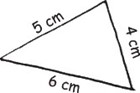
\includegraphics{img/triangleatracer2.jpg}
\end{exercise}
\end{multicols}

\begin{multicols}{2}
	\begin{exercise}
	Le triangle ci-dessous a été dessiné à main levée. Reproduis-le en respectant les mesures puis trace ses médiatrices. \\
	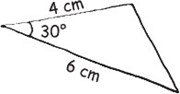
\includegraphics{img/triangleatracer3.jpg}
\end{exercise}

\begin{exercise}
	Le triangle ci-dessous a été dessiné à main levée. Reproduis-le en respectant les mesures puis trace ses bissectrices. \\
	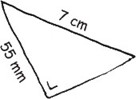
\includegraphics{img/triangleatracer4.jpg}
\end{exercise}
\end{multicols}

\begin{exercise}
	Sébastien a commandé 8BD. La facture s’élève à 78€ dont 6€ pour les frais d’envoi. Calcule le prix d’une BD. Laisse ta démarche visible.
\end{exercise}

\begin{exercise}
	Observe la suite suivante. \\ 
	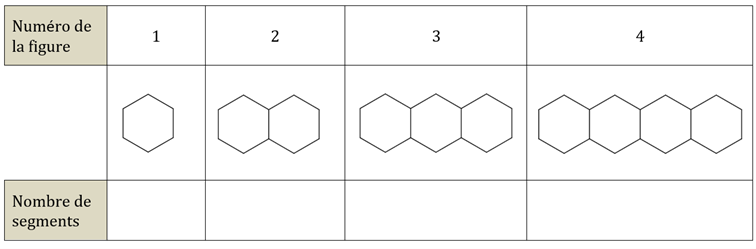
\includegraphics{img/suite.png}
	\begin{enumerate}
		\item \emph{(Sur cette feuille)} Complète le tableau. 
		\item Combien de segments constitueront la figure n°5 ?
		\item Quelle est la formule qui lie le numéro de la figure (\(n\)) au nombre de segments (\(s\)) ?
		\item De combien de segments sera constituée la figure n°10 ? 
		\item Quel est le numéro de la figure constituée de 56 segments? 
	\end{enumerate}
\end{exercise}

\begin{exercise}
	Une enquête a été réalisée au sein d’un école pour connaître le temps hebdomadaire moyen consacré au sport. Voici les résultats obtenus (en minutes) pour les six années. \\
	1ère année : 160 \hfill 2ème année : 310 \hfill 3ème année : 330 \hfill 4ème année : 120 \hfill 5ème année : 150 \hfill 6ème année : 70 \\
	Représente cette situation à l’aide d’un diagramme en bâtonnets.
\end{exercise}

\begin{exercise}
	Exprime en une expression littérale réduite le périmètre et l’aire des figures ci-dessous. \\  Détermine, ensuite, le périmètre de chaque figure si \(x=3\).\\
	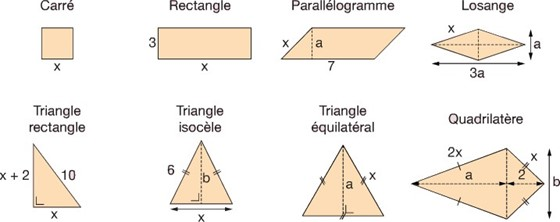
\includegraphics{img/PetA.jpg}
\end{exercise}

%%%%%%%%%%%%%%%%%%%%%%%%%%%%%%%%%%%%%%%%%%%%%%%%%%%%%%%%%%%%%%%%%%%%%%%%%%%%%%%%%%%%%%%%%%%%%%%%%%%%
%%SOLUTIONS 
%%%%%%%%%%%%%%%%%%%%%%%%%%%%%%%%%%%%%%%%%%%%%%%%%%%%%%%%%%%%%%%%%%%%%%%%%%%%%%%%%%%%%%%%%%%%%%%%%%%%
%\pagebreak
%\setcounter{nexo}{1}
%\textbf{Exercice \thenexo} \stepcounter{nexo}
\end{document}